% coding:utf-8

%FOSAET, a LaTeX-Code for a electrical summary of basic electronics
%Copyright (C) 2013, Daniel Winz, Ervin Mazlagic

%This program is free software; you can redistribute it and/or
%modify it under the terms of the GNU General Public License
%as published by the Free Software Foundation; either version 2
%of the License, or (at your option) any later version.

%This program is distributed in the hope that it will be useful,
%but WITHOUT ANY WARRANTY; without even the implied warranty of
%MERCHANTABILITY or FITNESS FOR A PARTICULAR PURPOSE.  See the
%GNU General Public License for more details.
%----------------------------------------

\chapter{Drehstrom}
\newpage
%\input{}
%
$U$: Aussenleiterspannung

$U_s$: Strangspannung
\[ U_s = \frac{U}{\sqrt{3}} \]
\[ \begin{array}{@{}l@{}l@{}l@{}r}
U_{1N} &= U_s &\angle &   0^\circ \\
U_{2N} &= U_s &\angle &-120^\circ \\
U_{3N} &= U_s &\angle & 120^\circ \\
U_{12} &= U   &\angle &  30^\circ \\
U_{23} &= U   &\angle & -90^\circ \\
U_{31} &= U   &\angle & 150^\circ 
\end{array} \]
\[ Y_1 = \frac{1}{Z_1} \]
\[ Y_2 = \frac{1}{Z_2} \]
\[ Y_3 = \frac{1}{Z_3} \]
\[ Y_n = \frac{1}{Z_n} \]
\[ U_{KN} = \frac{Y_1 \cdot U_{1N} + Y_2 \cdot U_{2N} + Y_3 \cdot U_{3N}}
{Y_1 + Y_2 + Y_3 + Y_N} \]
\begin{figure}[h!]
  \centering
  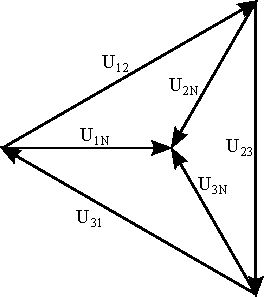
\includegraphics[width=0.3\textwidth]{../fig/drehstrom.pdf}
  \caption{Zeigerdiagramm Drehstrom}
  \label{fig:zeig_dreh}
\end{figure}
